\documentclass{beamer}
\usetheme{default}
\usecolortheme{dove}
\usepackage{setspace}
\usepackage[utf8]{inputenc}
\usepackage[russian]{babel}
\usepackage{array,caption}
\usepackage{amsmath}
\usepackage{gnuplottex}
\usepackage[absolute,overlay]{textpos}
\usepackage{graphicx}
\usepackage[percent]{overpic}
\usepackage{tikz}
\usetikzlibrary{shapes,positioning,shadows,trees,automata,arrows.meta,shapes.geometric}
\usepackage{setspace}
\usepackage{makecell}

\hypersetup{
  unicode=true
}

\title{\textbf{Serverless Computing}}
\subtitle{Подготовка к выполнению курсового задания}
\author[Author]{
    Титов А.И., СПбПУ ИПММ 6 курс
    \\
    Крутских А.О., СПбПУ ИПММ 6 курс
    \\
    Преподователь: Лукашин А.А.}
\date{}

\usenavigationsymbolstemplate{}
\setstretch{0.9}

\renewcommand{\arraystretch}{1.2}

\setbeamertemplate
{footline}{\footnotesize\quad\hfill\insertframenumber\hspace*{3ex} \vspace*{3ex}}
\setbeamertemplate{itemize item}{$\bullet$}
\setbeamertemplate{section in toc}{\inserttocsectionnumber.~\inserttocsection}
\setbeamertemplate{frametitle}{\textbf{\insertframetitle}\\ \textmd{{\insertframesubtitle}}}
\addtobeamertemplate{frametitle}{\vspace*{0.3cm}}

\begin{document}
    \addtobeamertemplate{headline}{}
    {
    \begin{textblock*}{100mm}(9.1cm, 5 mm)
        
\includegraphics[height=9mm]{images/POLYTECH}
    \end{textblock*}
    }

    \begingroup
    \renewcommand{\insertframenumber}{}
    \begin{frame}
        \vspace*{1.5cm}
        \addtocounter{framenumber}{-1}
        \titlepage
    \end{frame}
    \endgroup


    \begin{frame}
        \frametitle{Введение}
        \framesubtitle{Что такое <<Бессеррверные\\вычисления>>?}
        \textbf{Бессерверные вычисления} -- модель облачных вычислений, в которой ресурсы распределяются динамически самой платформой, организующей облако.
        \begin{figure}
            
\includegraphics[width=0.7\linewidth]{images/Logos}
        \end{figure}
    \end{frame}


    \begin{frame}
        \frametitle{Введение}
        \framesubtitle{Что такое <<Бессеррверные\\вычисления>>?}
        \begin{figure}
            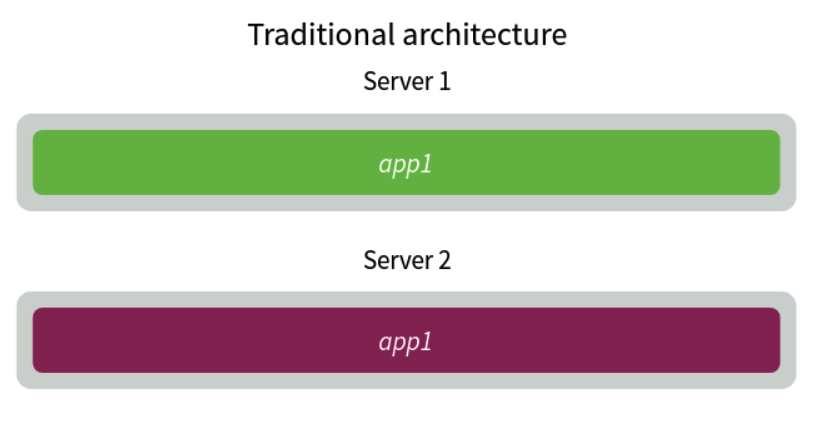
\includegraphics[width=0.6\linewidth]{images/Traditional}
        \end{figure}
        \vspace*{-0.6cm}
        \begin{figure}
            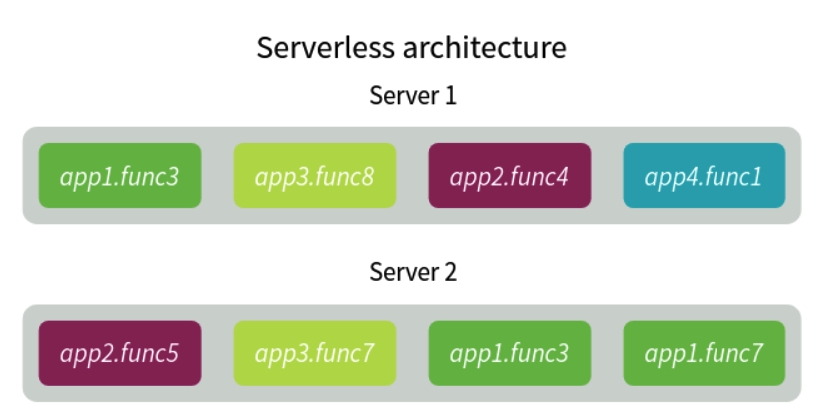
\includegraphics[width=0.6\linewidth]{images/Serverless}
        \end{figure}
    \end{frame}


    \begin{frame}
        \frametitle{Введение}
        \framesubtitle{Function as a service (FaaS)}
        \vspace*{-0.3cm}
        \begin{figure}
            \includegraphics[width=0.9\linewidth]{images/Faas}
        \end{figure}
    \end{frame}


    \begin{frame}
        \frametitle{Введение}
        \framesubtitle{Преимущества}
        \begin{itemize}
            \item Отсутствие процесса администрирования
            \item Pay-per-use
            \item Автоматическое масштабирование
            \item Скорость
        \end{itemize}
    \end{frame}


    \begin{frame}
        \frametitle{Amazon Web Services\\(AWS) Lambda}
        \framesubtitle{Возможности}
        Lambda запускает код в высокопроизводительной вычислительной среде и занимается административной поддержкой всех ресурсов, включая обслуживание серверов и операционных систем, распределение производительности, установку ПО и т.д.
        \vspace*{-0.6cm}
        \begin{figure}
            
\includegraphics[width=0.5\linewidth]{images/awslogo}
        \end{figure}
    \end{frame}


    \begin{frame}
        \frametitle{Amazon Web Services\\(AWS) Lambda}
        \framesubtitle{Возможности}
        \begin{tabular}{m{0.21\linewidth}m{0.78\linewidth}}
            {
            \footnotesize
            Языки SDK:
            \begin{itemize}
                \item Node.js
                \item Java
                \item Python
                \item Go
                \item C\#
                \item PowerShell
                \item Ruby
            \end{itemize}
            }
            &
            \centering
            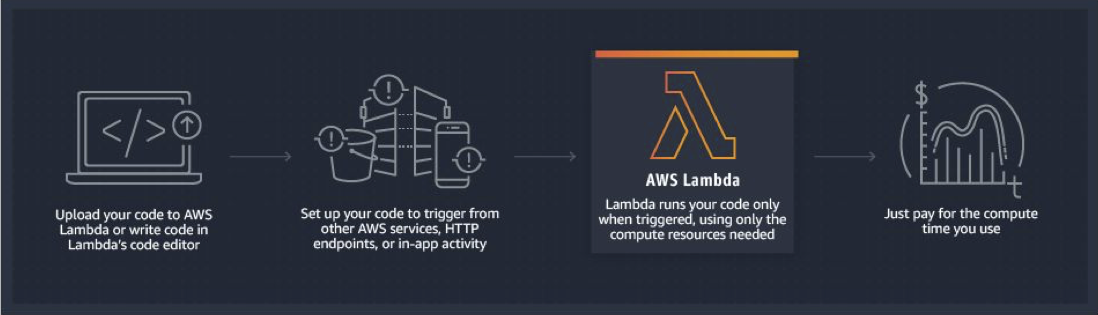
\includegraphics[width=\linewidth]{images/aws-opp}
 		\end{tabular}
        Также предоставляется API среда выполнения для создания функций с использованием любых других языков.
    \end{frame}


    \begin{frame}
        \frametitle{Amazon Web Services\\(AWS) Lambda}
        \framesubtitle{Цена}
        \begin{figure}
            
\includegraphics[width=\linewidth]{images/awsPrice}
        \end{figure}
        Плата взимается на основе количества запросов к функциям и их продолжительности, т. е. времени, в течение которого исполняется код.
    \end{frame}


    \begin{frame}
        \frametitle{Google}
        Компания Google имеет сразу две популярные платформы для бессерверных вычислений:

        \begin{itemize}
            \item Google Cloud Functions
            \item Firebase (Компания поглощена Google с 2014 г.)
        \end{itemize}

        \begin{figure}
            \includegraphics[width=0.3\linewidth]{images/Google}
        \end{figure}
    \end{frame}

    \begin{frame}
        \frametitle{Google Cloud Functions}
        \framesubtitle{Возможности}
        \begin{tabular}{m{0.18\linewidth}m{0.8\linewidth}}
            {
            \small
            Языки SDK:
            \begin{itemize}
                \item Node.js
                \item Python
                \item Go
            \end{itemize}
            }
            &
            \centering
            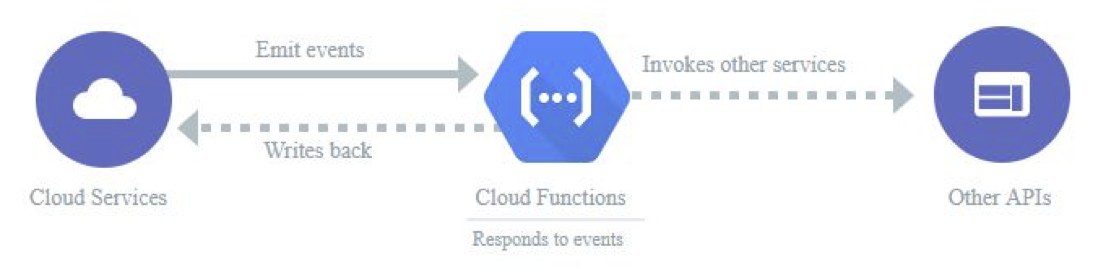
\includegraphics[width=\linewidth]{images/google-opp}
 		\end{tabular}
    \end{frame}


    \begin{frame}
        \frametitle{Google Cloud Functions}
        \framesubtitle{Цена}
        \begin{figure}
            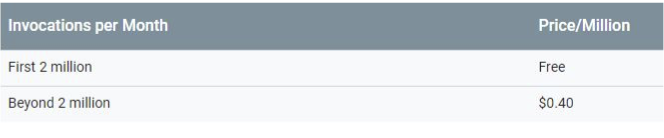
\includegraphics[width=\linewidth]{images/googlePrice-1}
        \end{figure}
        Цена зависит от того, как долго выполняется ваша функция, сколько раз она вызывается и сколько ресурсов вы выделяете для этой функции. Плата за время вычислений варьируется в зависимости от объема памяти и ЦП, выделенных для функции.
    \end{frame}

    \begin{frame}
        \frametitle{Google Cloud Functions}
        \framesubtitle{Цена}
        \begin{figure}
            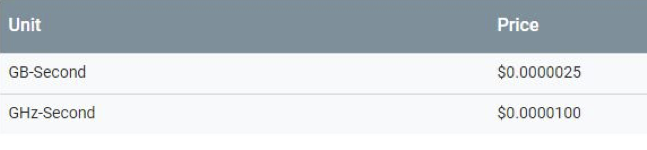
\includegraphics[width=\linewidth]{images/googlePrice-2}
        \end{figure}
        GCF предоставляют постоянный бесплатный уровень, который включает в себя выделение 2 млн вызовов, 400 000 ГБ-секунд, 200 000 ГГц-секунд вычислительного времени и 5 ГБ выходного интернет-трафика в месяц.\\
        Предоставляется кредит на 300 долларов США.
        \vspace*{0.5cm}
        {
        \tiny
        \begin{itemize}
            \item 1 GB-second - это 1 секунда времени с выделением 1 ГБ памяти
            \item 1 GHz-second - это 1 секунда времени  с выделенным процессором 1 ГГц
        \end{itemize}
        }
    \end{frame}


    \begin{frame}
        \frametitle{Firebase}
        \framesubtitle{Возможности}
        \vspace*{0.2cm}
        \begin{tabular}{m{0.47\linewidth}m{0.47\linewidth}}
            \centering
            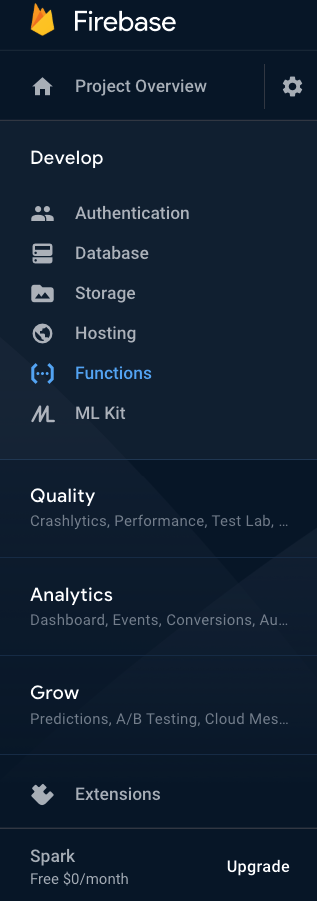
\includegraphics[width=0.5\linewidth]{images/FirebaseInterface}
            &
            Языки SDK:
            \begin{itemize}
                \item Node.js
                \item Java
                \item Python
                \item Go
                \item C\#
            \end{itemize}
 		\end{tabular}
    \end{frame}


    \begin{frame}
        \frametitle{Firebase}
        \framesubtitle{Цена}
        \begin{figure}
            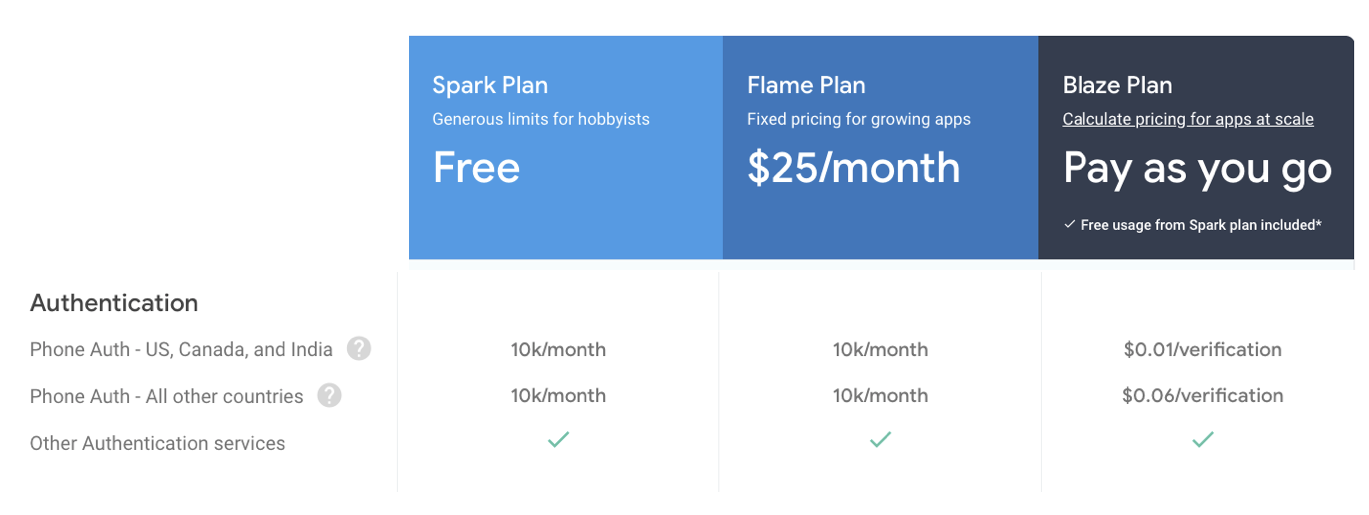
\includegraphics[width=\linewidth]{images/FirebasePrice}
        \end{figure}
        Blaze Plan также имеет бесплатный уровень - 2 000 000 вызовов, 400 000 Гб-сек., 200 000 ЦПУ-сек. и 5 Гб исходящего интернет-трафика предоставляется ежемесячно.
    \end{frame}


    \begin{frame}
        \frametitle{Microsoft Azure Functions}
        \framesubtitle{Возможности}
        \begin{tabular}{m{0.47\linewidth}m{0.47\linewidth}}
            Языки SDK:
            \begin{itemize}
                \item Node.js
                \item Python
                \item C\#
                \item F\#
                \item PHP
                \item batch
                \item bash
            \end{itemize}
            &
            \centering
            
\includegraphics[width=0.8\linewidth]{images/azurelogo}
 		\end{tabular}
    \end{frame}


    \begin{frame}
        \frametitle{Microsoft Azure Functions}
        \framesubtitle{Цена}
        \begin{figure}
            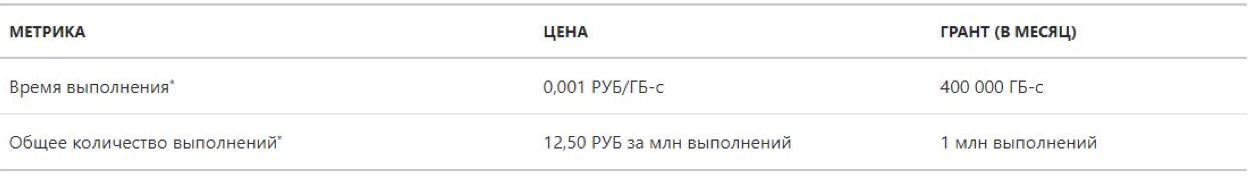
\includegraphics[width=1.05\linewidth]{images/azurePrice}
        \end{figure}
        Плата начисляется в зависимости от потребления ресурсов и числа выполнений в секунду. В цену плана потребления входит ежемесячный грант на 1 млн запросов и 400 000 ГБ/с.\\
        \vspace*{0.5cm}
        Бесплатная учетная запись:
        \begin{itemize}
            \item 1 млн запросов в месяц в MAF
            \item 12 500 руб на счет для изучения возможностей любой службы Azure в течение 30 дней
        \end{itemize}
    \end{frame}


    \begin{frame}
        \frametitle{Apache OpenWhisk}
        Облачная платформа с открытым исходным кодом.

        Популярные решения, основанные на технологии:
        \begin{itemize}
            \item IBM Cloud Functions
            \item RedHat OpenShift
        \end{itemize}

        Далее будут рассматриваться возможности Apache OpenWhisk на примере IBM Cloud Functions.

        \begin{figure}
            
\includegraphics[width=0.4\linewidth]{images/apache}
        \end{figure}
    \end{frame}


    \begin{frame}
        \frametitle{IBM Cloud Functions}
        \framesubtitle{Возможности}
        \begin{figure}
            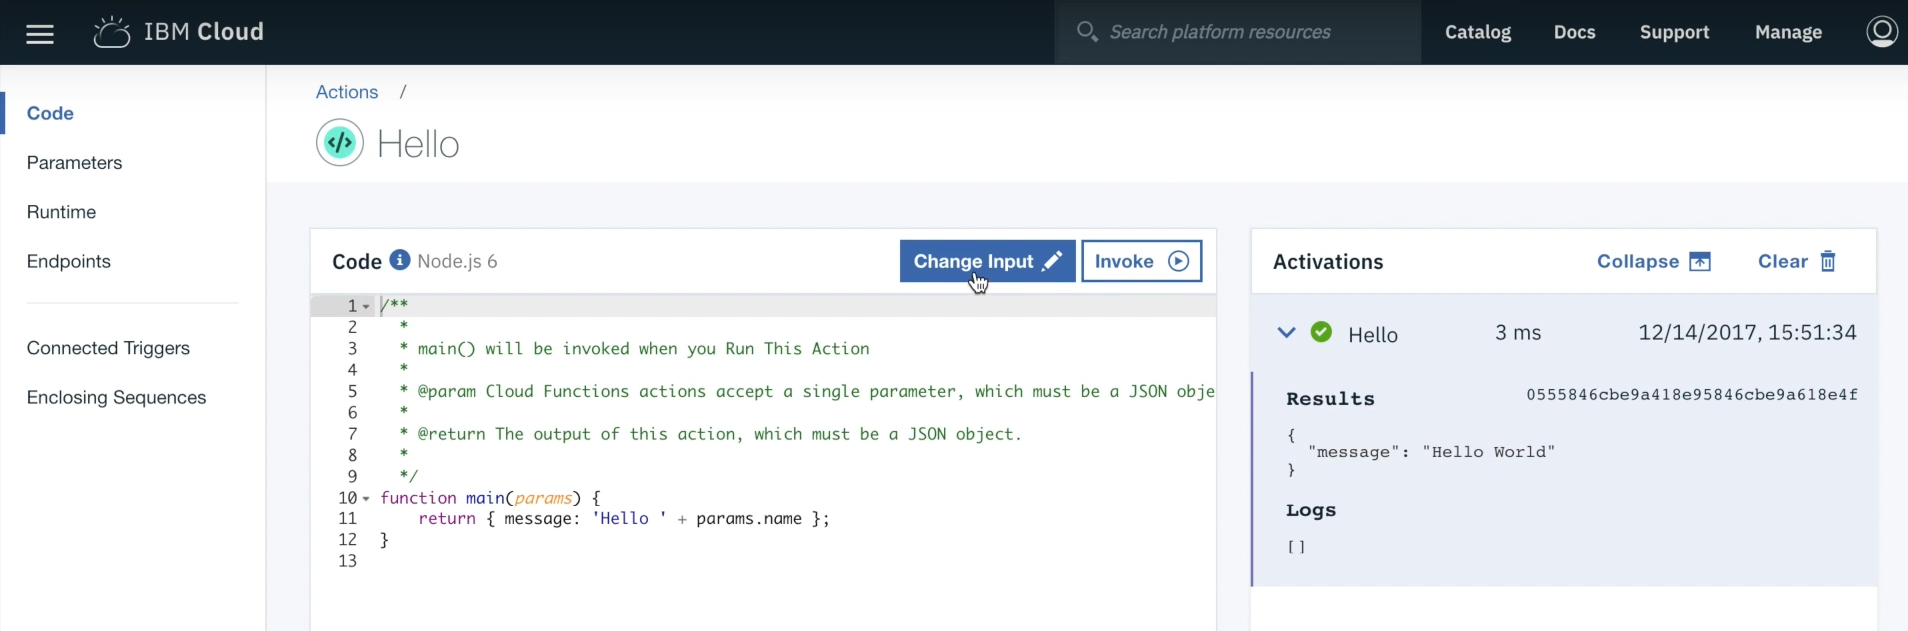
\includegraphics[width=1.05\linewidth]{images/ibmcloud}
        \end{figure}
        \vspace*{-0.5cm}
        Языки SDK:
        \begin{itemize}
            \item Node.js
            \item PHP
            \item Python
            \item Swift
        \end{itemize}
    \end{frame}


    \begin{frame}
        \frametitle{IBM Cloud Functions}
        \framesubtitle{Цена}
        \begin{figure}
            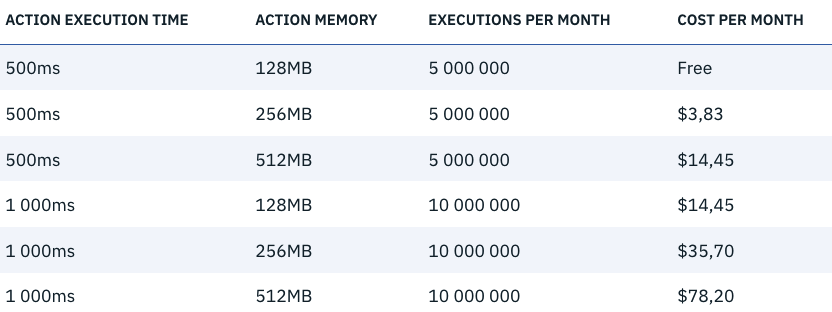
\includegraphics[width=\linewidth]{images/ibmprice}
        \end{figure}
        Присутствует программа Free-tier. Бесплатные условия отображены в таблице с примерами.
    \end{frame}


    \begin{frame}
        \frametitle{OpenStack}
        \framesubtitle{Qinling}
        В инфраструктуре OpenStack возможно организовать Serverless Computing с помощью проекта Qinling.
        \vspace*{0.5cm}
        Нативная поддержка:
        \begin{itemize}
            \item Основные платформы оркестрации (Kubernetes/Swarm, и др.)
            \item Основные хранилища данных (local/Swift/S3)
        \end{itemize}
        \vspace*{0.5cm}
        На домашней странице проекта приведено полное описание установки и использования.\\
        https://docs.openstack.org/qinling/latest/
    \end{frame}


    \begingroup
    \setbeamertemplate
    {footline}{}
    \begin{frame}
        \addtocounter{framenumber}{-1}
        \center
        \Large{Спасибо за внимание!}
    \end{frame}
    \endgroup
\end{document}